\documentclass[11pt]{amsart}
\usepackage[utf8]{inputenc}
\usepackage{fullpage}
\usepackage{floatrow}
\usepackage{amsmath,amssymb,amsthm}
\usepackage{verbatim}
\usepackage{listings}
\usepackage{enumerate}
\usepackage{hyperref}
\usepackage{dsfont}
\usepackage{mathtools}
\usepackage{caption}
\usepackage{subcaption}
\usepackage{booktabs}
\usepackage[table]{xcolor}
\usepackage[margin=1in]{geometry} 

%\renewcommand{\slimits@}{\limits}
%\renewcommand{\nmlimits@}{\limits}

\newcommand{\RN}{\mathbb{R}^n}
\newcommand{\Cx}{\mathbb{C}}
\newcommand{\Sp}{\mathbb{S}}

\newcommand{\zbar}{\overline{z}}
\newcommand{\C}{\mathbb{C}}
\DeclareMathOperator{\im}{Im}
\DeclareMathOperator{\re}{Re}
\newcommand{\pd}[2]{\frac{\partial #1}{\partial #2}}
\newcommand{\R}{\mathbb{R}}
\newcommand{\N}{\mathbb{N}}
\newcommand{\E}{\mathbb{E}}
\newcommand{\var}{\text{Var}}
\newcommand{\Mod}[1]{\ (\mathrm{mod}\ #1)}
\newcommand{\cov}{\text{Cov}}
\newcommand{\G}{\mathcal{G}}
\newcommand{\Lbar}[1]{\overline{L_{#1}}}
\newcommand{\boxb}{\square_b}
\newcommand{\LB}{\Delta_{\Sp^{2n-1}}}
\newcommand{\hpq}{\mathcal{H}_{p,q}(\Sp^{2n-1})}

\usepackage{graphicx}

\newtheorem{theorem}{Theorem}
\newtheorem{remark}{Remark}
\newtheorem{lemma}[theorem]{Lemma}
\newtheorem{proposition}[theorem]{Proposition}
\newtheorem{corollary}[theorem]{Corollary}
\newtheorem{conjecture}[theorem]{Conjecture}
\numberwithin{equation}{section}
\numberwithin{figure}{section}
\numberwithin{theorem}{section}
\newtheorem{example}{Example}
\newtheorem*{theorem*}{Theorem}
\newtheorem*{definition*}{Definition}
\newcommand{\Var}{\textnormal{Var}}

\setlength{\intextsep}{10pt minus 10pt}
\title[title]{Incarcerations By Race and Gender in 2002}
\author{Manuel F Perez}
\begin{document}
\maketitle

In this brief report, I explore trends in incarceration rates and lengths by race and gender in the United States in 2002. I use data from the National Longitudinal Surveys provided sponsored by the Bureau of Labor Statistics. Specifically, the dataset I use records the months during which various respondents were incarcerated in 2002. I sum the number of months incarcerated for each individual to obtain a dataset that consists of demographic indicators for race and gender, along with the number of months incarcerated during 2002. The figure and table below shows a summary of the mean months of incarceration by race and gender:

\begin{figure}[H]
    \centering
    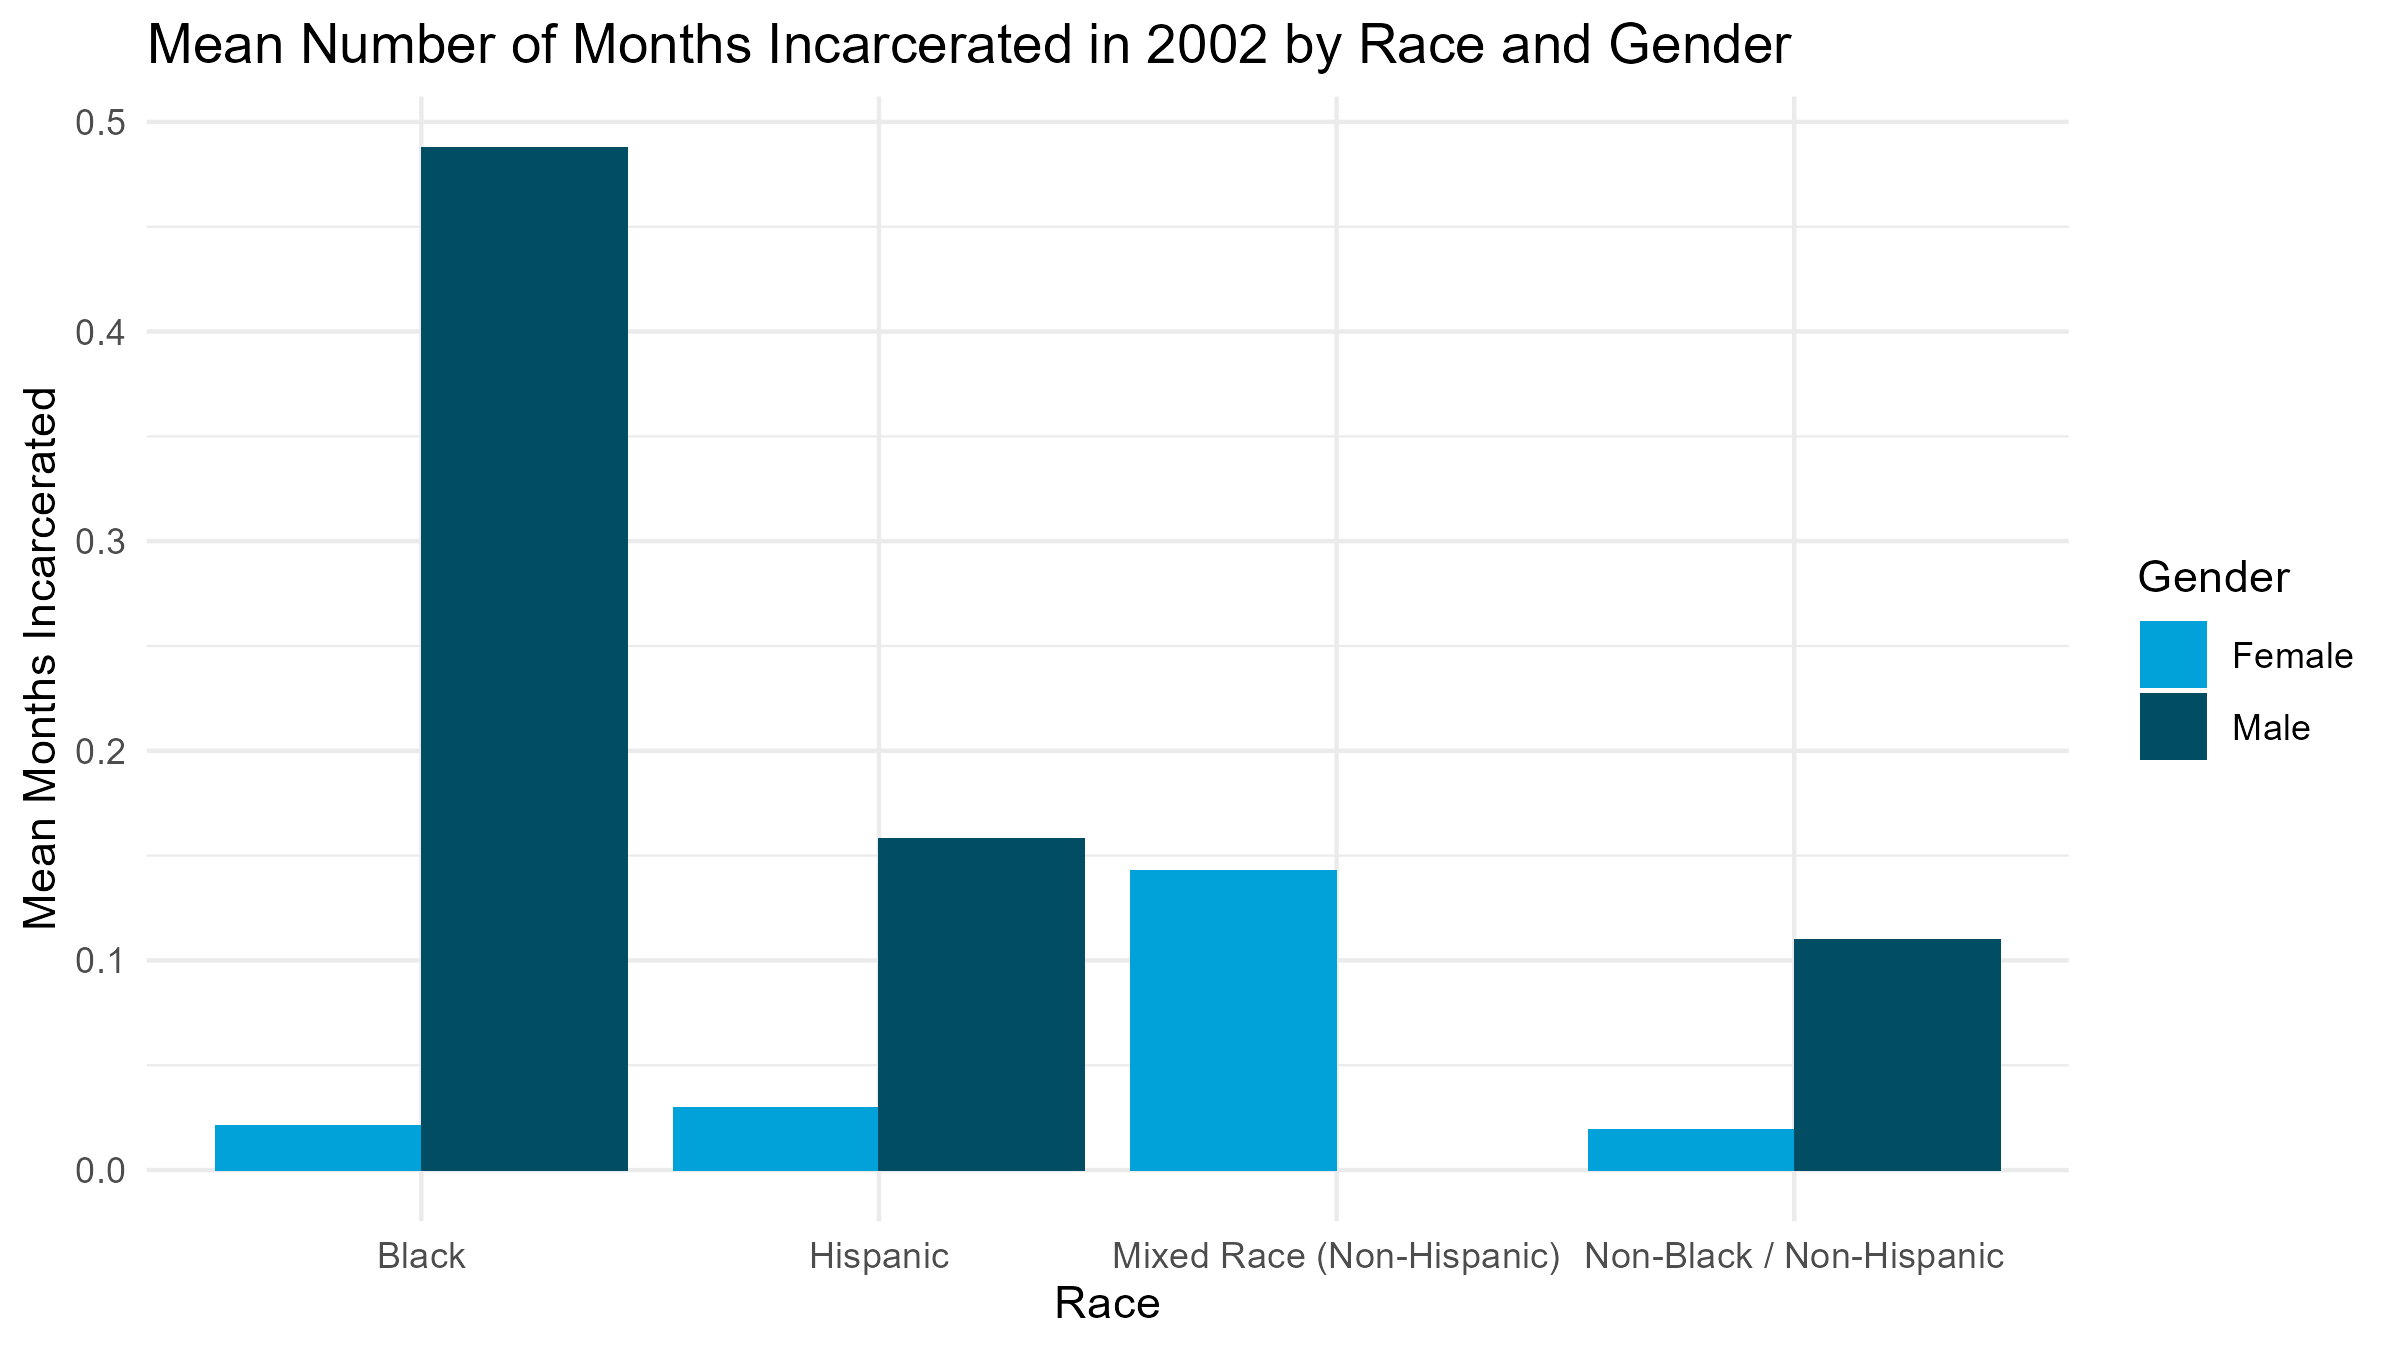
\includegraphics[scale=0.8]{incarceration_by_racegender.png}
\end{figure}

\begin{table}[H]

\caption{\label{tab:tab:summarystats}Mean months incarcerated in 2002 by Race and Gender}
\centering
\begin{tabular}[t]{lrrrr}
\toprule
Gender & Black & Hispanic & Mixed Race Non Hispanic & Non Black Non Hispanic\\
\midrule
\cellcolor{gray!6}{Female} & \cellcolor{gray!6}{0.0211268} & \cellcolor{gray!6}{0.0298013} & \cellcolor{gray!6}{0.1428571} & \cellcolor{gray!6}{0.0193192}\\
Male & 0.4876712 & 0.1579509 & 0.0000000 & 0.1099476\\
\bottomrule
\end{tabular}
\end{table}


We see that Black males are (by a wide margin) more likely to be incarcerated during any given time in 2002 compared to both Hispanic and Non-Black/Non-Hispanic males. We note that data on Mixed Race (Non-Hispanic) Males is either not plentiful enough, or was dropped during the data cleaning process, which prevents any further comparisons between this and other groups. For females, the incarceration likelihood seems to be very uniform if we assume, again, that the data on the Mixed Race (Non-Hispanic) group is too small/spurious to be reliable. This is not a robust analysis, but may lend credibility to the idea that Black Males bear the largest burden when it comes to racial bias in the justice system and/or socioeconomic circumstances that are correlated with crime.

In order to more robustly analyze these results, I regress months incarcerated on race and gender indicators, where Black Females are the omitted category:

\begin{table}[!htbp] \centering 
  \caption{Regression Output. Omitted category is Black Females.} 
  \label{tab:regression} 
\begin{tabular}{@{\extracolsep{5pt}}lc} 
\\[-1.8ex]\hline 
\hline \\[-1.8ex] 
 & \multicolumn{1}{c}{\textit{Dependent variable:}} \\ 
\cline{2-2} 
\\[-1.8ex] & Months Incarcerated in 2002 \\ 
\hline \\[-1.8ex] 
 Hispanic & $-$0.159$^{***}$ \\ 
  & (0.038) \\ 
  & \\ 
 Mixed Race (Non-Hispanic) & $-$0.174$^{**}$ \\ 
  & (0.083) \\ 
  & \\ 
 Non-Black / Non-Hispanic & $-$0.189$^{***}$ \\ 
  & (0.035) \\ 
  & \\ 
 Male & 0.194$^{***}$ \\ 
  & (0.022) \\ 
  & \\ 
 Constant & 0.155$^{***}$ \\ 
  & (0.026) \\ 
  & \\ 
\hline \\[-1.8ex] 
Observations & 8,621 \\ 
R$^{2}$ & 0.015 \\ 
Adjusted R$^{2}$ & 0.014 \\ 
Residual Std. Error & 1.019 (df = 8616) \\ 
F Statistic & 32.033$^{***}$ (df = 4; 8616) \\ 
\hline 
\hline \\[-1.8ex] 
\textit{Note:}  & \multicolumn{1}{r}{$^{*}$p$<$0.1; $^{**}$p$<$0.05; $^{***}$p$<$0.01} \\ 
\end{tabular} 
\end{table} 

This confirms the idea that female incarceration terms did not vary very widely by race in 2002. It also tells us that the average Black Male spent 0.189 more months incarcerated compared to the average Non-Black/Non-Hispanic Male, whereas the average Hispanic Male only spent 0.03 more months incarcerated compared to the average Non-Black/Non-Hispanic Male, pointing to a wide and alarming discrepancy in incarceration likelihood between Black Males and other groups.

\end{document}

